\documentclass[11pt,DIV=12]{scrreprt}

\usepackage{layout}

\makeglossaries

\newglossaryentry{REST}
{
	name=REST,
	description={\textbf{Re}presentational \textbf{S}tate \textbf{T}ransfer ist ein Programmierparadigma was sich häufig in Web Applikationen wiederfindet und generell das HTTP Protokoll verwendet.}
}

\newglossaryentry{BPM}
{
	name=BPM,
	description={\textbf{B}usiness \textbf{P}rocess \textbf{E}ngine ist eine Software, Bibliothek welche es erlaubt Geschäftsprozesse zu definieren und auszuführen.}
}

\newglossaryentry{RDBMS}
{
	name=RDBMS,
	description={\textbf{R}elational \textbf{D}ata\textbf{b}ase \textbf{M}anagement \textbf{S}ystem sind Datenbank Systeme welche sich an den relationel Prinzipien orientieren.}
}

\newglossaryentry{NoSQL}
{
	name=NoSQL,
	description={\textbf{N}ot only \textbf{SQL} sind Datenbanken welche sich nicht mehr an die relationalen Prinzipien halten und dadurch alternative Speicher formen für Daten ermöglichen. Die bekanntesten Typen sind Key-Value, Spalten-Orientiert, Dokumente-Orientiert und Graphen. NoSQL Datenbank besitzen im Vergleich zu relationalen Datenbanken kein Schema.}
}

\newglossaryentry{ACID}
{
	name=ACID,
	description={\textbf{A}tomicity \textbf{C}onsistency \textbf{I}solation \textbf{D}urability sind merkmale von relationalen Datenbanken welche stark auf Datenkonsitzenz setzen welches vorallem für Systeme im Finanzbereich unerlässlich sind.}
}

\newglossaryentry{BASE}
{
	name=BASE,
	description={\textbf{B}asically \textbf{A}vailable \textbf{S}oft-State \textbf{E}ventual Consitency ist ein Paradigma welches bei NoSQL Datenbanken anwendung findet. Die Konsitzenz wird dabei gegen vertikal Skalierbarkeit und Partitionierung getauscht.}
}

\newglossaryentry{Container}
{
	name=Container,
	description={Container sind in sich geschlossene Pakete welche ein Betriebsystem und Software enthalten. Sie laufen isololiert auf einem Hostsystem und haben keinen Zugriff auf dieses. Durch die Paketierung können die Container auf verschiedenen Linux Betriebsysteme laufen ohne das darunter liegende System zu beinflussen.}
}

\newglossaryentry{CAP-Theorem}
{
	name=CAP,
	description={\textbf{C}onsitency \textbf{A}vailability \textbf{P}artition Tolerance Theorem ist eine Klassifizierung für verteile System. Die Kernaussage ist, das ein System nur zwei der drei Charakteristiken gleichzeitig anbieten kann. Vor allem im Zuge von NoSQL wurde das Theorem wieder aufgegriefen. Es gibt einen einfachen Überblick jedoch sind verteilte System weit komplexer als dargestellt.}
}

\newglossaryentry{Kunde}
{
	name=Kunde,
	description={Eine Person welche mit der SIX eine Geschäftsbeziehung eingehen möchte um seinen Kunden Twint anbieten zu können.}
}

\newglossaryentry{PEP}
{
	name=PEP,
	description={\textbf{P}oliticaly \textbf{E}xposed \textbf{P}erson ist eine Person welche ein politisches Amt ausübt und deshalb in der Öffentlichkeit bekannt ist. Für diese Personen ist eine spezielle Prüfung notwendig.}
}


\begin{document}

\subject{Template}
\title{Masterthesis}
\author{Andreas Heubeck}
\date{\today}

\maketitle

\tableofcontents

\chapter{Management Summary}

Die vorliegende Masterthesis hat das Ziel eine Software Architektur zu entwerfen welche es erlaubt die darauf basierende Applikation, ohne Unterbruch des Dienstes, in einer produktiven Umgebung vollautomatisch zu installieren.\newline\newline
Neue Anforderungen, welche in immer kürzerer Zeit dem Benutzer zur Verfügungen gestellt werden müssen, sind eine neue Herausforderungen für den Finanzdienstleister SIX und die Motivation dieser Arbeit.\newline\newline
Methodisch orientierte sich das Vorgehen an Standard-Prozessen der Firma wie Scrum und Prototyping. Die neuen Anforderungen wurden mit dem Product Owner in Qualitätsszenarien für die neue Architektur übertragen. Die Problematik wurde zuerst in kleinere Teilprobleme aufgeteilt  für welche in einem weit gefassten Lösungsraum Varianten gesucht. Diese wurden mittels, einer mit dem Product Owner erarbeiteten Matrix, bewertet und bei Unklarheiten mit Prototypen verifiziert. Die daraus entstandenen Teillösungen sind mit der bestehenden Architektur zusammengeführt und die endgültige Lösung in einem Software Architektur Dokument spezifiziert worden. Das Dokument diente als Vorlage für den finalen Prototyp mit welchem die Qualitätsziele verifiziert wurden.\newline\newline
Diese Masterthesis zeigt zum Schluss auf, dass die gesetzten Qualitätsziele und Anforderungen, durch gezielten Einsatz von Methoden und Technologien, umgesetzt werden können und was die Folgen für SIX sind.

\chapter{Einleitung}

\section{Problemstellung}

Im Zuge der Digitalisierung ist es für Finanzdienstleister unerlässlich die angebotenen Dienstleistungen schneller weiterzuentwickeln und der Kundschaft bereitzustellen. Vor Allem bei Online-Diensten wird diese immer wichtiger. Mit der Entwicklung von Paymit war eine Lösung notwendig welche es potenziellen neuen Händler einfach erlaubt sich für den neuen Dienst anzumelden. Aus dieser Anforderung ist die Applikation Merchant Onboarding entstanden welches einem neuen Kunde erlaubt sich einfach über eine Web-Oberfläche zu registrieren.

Die Applikation wurde basierend auf neueren Technologien und Methoden entwickelt, welche es erlauben die Applikation schneller von der Entwicklung in die Produktion zu bringen. Im Vergleich zu normalen Releasezyklen von drei Monaten ist diese ein grosser Schritt forwärt.

Obschon die Applikation mittlerweile innert Tagesfrist ausgerollt werden kann, soll mit der Anpassung der Architektur auf Continuous Deployment \footnote{Methode welche es der Entwicklung und dem Betrieb erlaubt, eine Applikation automatisch nach jedem Code Commit neu auf den produktiven System zu installieren.} noch einen Schritt weiter gegangen werden. Um dieses Ziel zu erreichen, muss die Architektur der Applikation, mit dem Schwerpunkt Kommunikation zwischen der Teilen, angepasst werden. Des Weiteren sind gegebenefalls Änderungen an Processen wie Change Managemen notwendig.
Der Vorteil dieses Ansatzes erlaubt es, Fehler oder Erweiterungen nach einem standartisierten und automatischen Prozess ohne menschliche Intervention zu installieren. Dadruch kann die Firma sehr schnell auf sich änderne Anforderungen reagieren.


\section{Systemabgrenzung}

Finanzdienstleiter wie die SIX haben für die Abwicklung ihres Geschäfts eine grosse Anzahl Applikation welche verschiedene Geschäftstätikeiten abdecken. Auch das Merchant Onboarding ist ein Teil dieser Landschaft und kann nur durch Interaktion mit diesen System seine Aufgabe erledigen. In der folgenden Tabelle sind kurz die Systeme aufgeführt welche Merchant Onboaring verwendet, jedoch nicht Teil der Problemstellung und Lösung sind.

\begin{table}[H]
	\centering
	\caption{Verwendete Applikationen}
	\begin{tabular}{ | p{2cm} | p{14cm} | }
		\toprule
		{\textbf{Applikation}} & {\textbf{Beschreibung}} \\
		\midrule
		PASS & \textbf{P}ayment \textbf{A}cquiring \textbf{S}ervices \textbf{S}ystem. Applikation welche die Transaktionen verarbeitet und Händlerauszahlungen auslöst. \\ \hline
		Workflow Engine & Business Process Engine welche sich die Erstellung des Kundenkontos kümmert.\\ \hline
		SCS & Registrationstelle für neue Zahlungsterminal.\\ \hline
		ZEFIX & Schnittstelle zum Handelsregister\\ \hline
		AddressService Post\\ \hline
		Google Maps\\ \hline
		ATMS Service (MTAN)\\
		\bottomrule
	\end{tabular}
\end{table}

Des Weiteren gibt es Teile der Infrastruktur welche die Lösung tangieren im Hinblick auf deren Aktualisierung welche aber nicht Berücksichtigt werden da es sich beim Thema um die Architektur der Anwendung geht. Diese sind in der folgenden Tabelle kurz aufgeführt.

\begin{table}[H]
	\centering
	\caption{Infrastruktur}
	\begin{tabular}{ | p{2cm} | p{14cm} | }
		\toprule
		{\textbf{Komponente}} & {\textbf{Beschreibung}} \\
		\midrule
		Betriebsystem & Die Basis auf welcher die Applikaton läuft ist nicht Bestandteil der Architektur. \\ \hline
		Netzwerk & Netzwerkkomponenten wie Switches, Router, Storage und der gleiche sind auch mit Software augestattet, werden jedoch nicht berücksichtigt.\\ \hline
		Datenbank Software & Die automatische Aktualisierung ist nicht Teil der Architektur. Obschon patches meist automatisch eingespielt werden können, ist bei Major Versionen dies meistens mit mehr Aufwand verbunden. \\ \hline
		BPM Engine & Die Prozess Verarbeitung basiert auf einem Produkt welches akutell noch nicht die Möglichkeit für Continuous Delivery besitzt. Deshalb wird diese Komponente nur bezüglich Schnittstellen berücksichtigt.\\
		\bottomrule
	\end{tabular}
\end{table}



\graphicspath{{./images/}}

\chapter{Ausgangslage}

\section{Ist-Zustand}

Die Applikation ist aktuell seit xxx in Betrieb und wird regelmässig erweitert. 

Die Applikation MEON wird aktuell mittels Continuous Delivery \footnote{Methode welches es der Entwicklung erlaubt Applikationen schnell auf nicht produktiven System auszurollen.} auf interne Testsysteme installiert. 

\section{Situationsanalyse}

Für die Umsetzung der Masterthesis wird Scrum verwendet. Scrum ist eine Agile Vorgehensmethodik welche nur wenige Regeln vorgibt. Die Wahl fiel auf diese Methodik da sie erstens sehr schlank ist und schnelle Feedbackzyklen erlaubt wodurch die Lösung besser auf die Bedürfnisse der Stakeholder abgestimmt werden kann. Des Weiteren können Probleme und Risiken dadurch früher entdeckt werde. Scrum ist in der Abteilung, in welcher die Masterthesis gemacht wird, die Standard Methodik für Software Projekte. Dabei werden nicht nur Entwicklungs- sondern auch, Analyse-, Anforderungs- und Testaufgaben damit abgehandelt. Die Position des Product Owners wird von meinem Betreuer eingenommen. Die Sprintdauer wird auf zwei Wochen angesetzt. Da die Masterthesis eine Einzelarbeit ist, werden andere Scrum Prozesse wie Retrospektive und Planning entsprechen vereinfacht oder ganz weggelassen. Scrum bietet den Rahmen für das Erstellen eines Software Architektur Dokumentes auf der Basis von Arc42.
Prototyping soll verwendet werden um die ausgewählten Lösungsstrategien gegenüber den Anforderungen zu verifizieren und gegebenenfalls anzupassen.  

Im vergleich zu anderen Projekte sehr modern

\graphicspath{{./images/}}

\newgeometry{left=2.5cm, right=2.5cm, bottom=2.5cm, top=2.5cm}

\begin{landscape}
	
\chapter{Projektmanagement}

Obschon ein iteratives Vorgehen wie Scrum als Methode für die Erarbeitung der Masterthesis verwendet wird, ist es für den Überblick der Arbeit unumgänglich eine groben Projektplan vorliegen zu haben. Neben dem Plan wurden auch allfällige Risiken und die damit verbundenen Massnahmen aufgelistet. Diese beziehen sich auf Risiken für die Umsetzung der Thesis und des Umfeldes. Im Software Architektur Dokument Im Kapitel 11 sind die technischen Risiken der Architektur aufgeführt.


\section{Projektplan}

Der Projektplan wurde grob gehalten und nur die wichtigsten Aufgaben aufgenommen um den Plan nicht zu überladen. Die Reserve am Schluss dient als Puffer falls sich trotz der Planung Probleme ergeben sollten.

\begin{figure}[H]
	\centering
	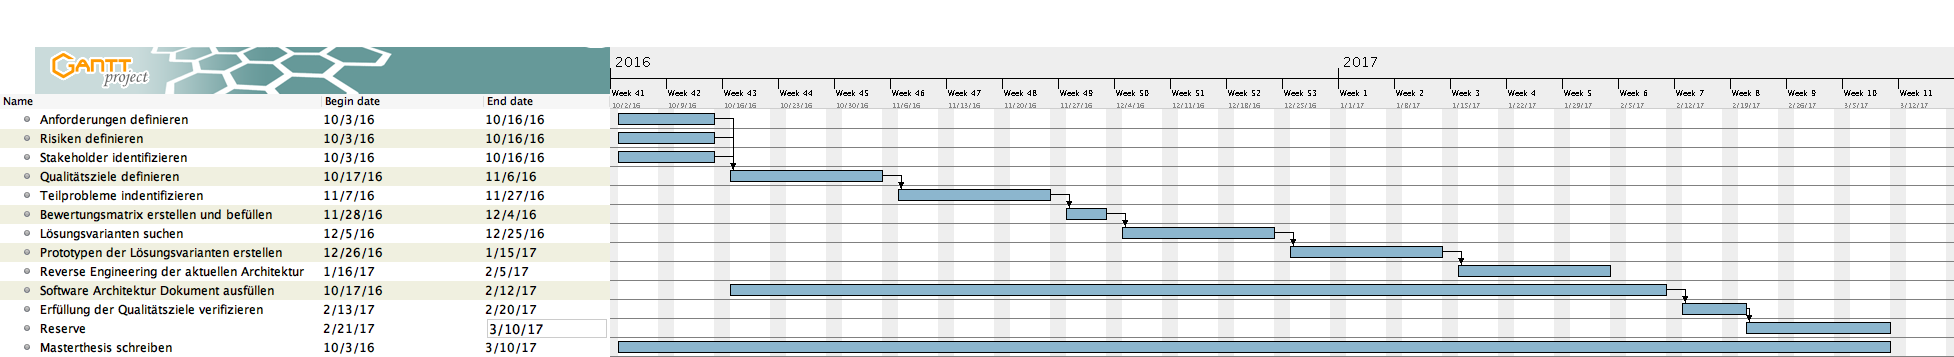
\includegraphics[scale=0.37]{projectplan.png}
	\caption{Projektplan}
\end{figure}
\newpage	

\section{Risiken}
\begin{table}[h!]
	\centering
	\caption{Risiken}
	\begin{tabular}{ | p{2cm} | p{10cm} | p{10cm} | }
		\toprule
		{\textbf{Risiko}} & {\textbf{Beschreibung}} & {\textbf{Massnahmen}} \\
		\midrule
		Richtlininen der Firma & Abklärungen und Vorschläge wie die Richtlinien eingehalten werden können oder angepasst werden müssten. & Die bestehenden Richtlinien werden von der Applikation bereits eingehalten. Die Vorgaben bezüglich Change Management müssen frühzeitig angegangen werden da es Einfluss auf den Prozess hat. \\ \hline
		Conway's law & Conway's law ist eine Beziehung zwischen der Firmenorganisation und der Softwarearchitektur. Das Gesetz besagt, dass die Software Architektur eines Systems sich nach der Firma richtet. & Obschon die Organisation noch eher klassisch aufgebaut ist, sind durch firmeninterne Initiativen die Entwicklungsabteilungen nicht so stark an Vorgaben gebunden. Dennoch ist das Risiko im Auge zu behalten. \\ \hline
		Fehlende Requirements & Das Projekt wurde in kurzer Zeit umgesetzt und hat deshalb keinen formalen Requirement Engineering Prozess durchlaufen. Dadurch sind weder funktionale noch nicht funktionalen Anforderungsdokumente vorhanden. &  Da die Applikation überschaubar ist und einen klaren Business Case hat, werden die aktuellen Anforderung nach getragen damit durch Anpassungen an der Architektur keine Fachlichkeit geändert wird. \\ \hline
		Neue Requirements & Die Requirements für die Architekturanpassung sind nicht definiert. & Da die Anforderung von der Entwicklungsabteilung getrieben wird, sollen die Basisanforderungen als erstes erfasst werden. Änderungen oder Ergänzungen sollen nach-dokumentiert werden.\\
		\bottomrule
	\end{tabular}
\end{table}

\end{landscape}
\restoregeometry

\chapter{Ausgangslage}

\chapter{Lösung}

\section{Requirements}

Unternehmensarchitekten zu weit weg vom geschene deshalb als Stakeholder weg

\section{Kontextabgrenzung}

Wie wurde die Lösung erarbeitet. Das Was ist im SAD obschon gewisse Teile zusammengefasst hier aufgeführt werden müssen.

erarbeiten der Anforderungen und den Qualitätszielen. MEON exisitiert bereits keine alten Anforderungen vorhanden. 

Qualitätsziele und neue Anforderungen nicht einfach definierbar da aktuell gar nicht klar wie das überhaupt ausehen soll. Anforderungen deshalb pro forma mal aufgenommen mit der Möglichkeit diese später anzupassen.
Organisatorischer Teil impact weitgehend unklar da das Projekt dies bezüglich grössere freiheiten genossen hat. 

\section{Qualitätsziele}

\section{Teilprobleme}

- Pipeline
- Versionierung
- Asynchronität
- Datenspeicherung
- Konfigurationsmanagement

\section{Teillösungen}

Diverse Teilösungen indentifiziert anhand der bis zu diesem Zeitpunkt vorhandenen Requirements -> Qualitätsziele nach wievor nicht komplett klar.
Möglichst grosser Lösungsraum an Teilprobleme um eine gute Sicht auf das zu lösende Problem zu bekommen.


Erstellen der Bewertungskriterien.

Bewerungskriterien erstellt und entsprechend aufgeführt.

Prototypen erstellen für die Unklarheiten der ausgewählen Teillösungen.

Bild erstellen für Problem der Datenmigration resp. der unterstützung von zwei gleichzeitig laufenden versionen.
RDBMS -> trigger recursion, migration
NoSQL -> kein schema jedoch gleiches problem

CAP Theorem

MySQL CA, Mongo CP

Beide Datenbankentypen erlauben das Problem zu lösen. RDBMS braucht die ändernung an zwei stellen-> Buch über alle möglichen Variationen. Zyrkuläre Trigger tükisch. Mongo: alle muss in Code gemacht werden. Ermöglich schrittweise migration


Evaluation Graphql
Content Negogiation und Versionierung nicht im Prototyp abgebildet da bereits hinreichend bekannt.
Graphql sehr mühesam für Mutationen nicht die gleiche Konfiguration wie für die Abfragen verwendet werden kann.Übergabe wie MAp was sehr viel casten verursacht.. Library nicht von einer Organisation entwickelt sondern von 36 Entwicklern über Github. Gelegentliche Commits jedoch nicht wirk lebendig. 

\section{Lösungsvariante}

\section{Bewertung}













\chapter{Erkenntnisse}

Während der Masterthesis wurden diverse Erkenntnisse gewonnen welche folgend kurz dargestellt werden.\newline

Scrum als gewählte Methode für die Abwicklung der Masterthesis hat sich nur bedingt bewährt. Das iterative Vorgehen und die ständige Kommunikation mit den Beteiligten Personen und dem Betreuer haben geholfen die Thesis effizient abzuwickeln und Probleme früh zu erkennen was von Vorteil war. Als Einzelperson bewähren sich die anderen Aspekte wie Planning und das vorbereiten von User Stories gemessen am Nutzen nicht. Eine Schwierigkeit ist auch das erstellen von Schätzungen wenn es um Schreiben von Text geht. Schlussendlich wurde eine einfach Checkliste verwendet um die Aufgaben zu verfolgen.\newline

Der Übergang von der Entwicklerrolle in die Architektenrolle hat gezeigt, dass nicht mehr alles genau Ausgearbeitet werden kann. Das Finden des richtigen Detaillevels ist wichtig um die Architektur nicht zu überladen, tendiert man als Entwickler doch dazu die Dinge genau verstehen zu wollen. Obschon es sich um eine Einzelarbeit handelte, musste öfters der Rat von Experten eingeholt werden, was zeigt, dass Vertrauen und Verlassen in seine Umgebung und deren Fähigkeiten ein wichtiger Bestandteil der Arbeit ist. Das entwerfen einer neuen Architektur hat auch gezeigt, dass ein gewisser Erfahrungsschatz an Methoden und Technologien vorhanden sein muss. Das generelle Interesse an der Informatik und damit verbundene Weiterbildungen sind faktisch Pflicht da sich ohne diese verschiedene Perspektiven auf Probleme gar nicht öffnen. Das Sprechen der verschiedenen Sprachen der Stakeholder ist am Anfang ungewohnt und bedarf Übung eröffnet aber eine ganzheitlichere Sicht auf Problemstellungen.\newline

Die wichtigste Erkenntnis ist, dass sich durch methodisches iteratives Zusammenarbeiten und klare Kommunikation ein, auf den ersten Blick komplexes Problem, gezielt lösen und dokumentieren lässt.

\chapter{Schlussfolgerung}

Die definierte Architektur hat die Anforderungen und die Qualitätsziele erfüllt und gezeigt, dass Continuous Deployment innerhalb von SIX möglich ist. Die gewonnen technischen Erkenntnisse können nun für Merchant Onboarding verwendet und sogar auf andere Projekte übertragen werden. Zusammen mit den bereits gestartete Veränderungen in der Kultur, die Verwendung von angemessenen Technologien und das Überdecken von alten Prozessen, könnte SIX seinen Kunden in Zukunft neue Funktionen, Fehlerbehebungen und sogar komplett neue Anwendungen in kurzer Zeit zu Verfügung stellen.\newline
Das Software Architektur Dokument, im speziellen das Arc42 Template, hat sich als gutes Mittel bewährt um die Anwendung auf einer mittleren Abstraktionsebene zu beschreiben. Ein Dokument alleine kann aber die Kommunikation der Architektur an die Entwickler nicht ersetzten. Der Architekt muss deshalb die Zusammenarbeit suchen um das Projekt schlussendlich zum Erfolg zu bringen.

\chapter{Massnahmen}

Da die komplette Installation von OpenShift noch nicht abgeschlossen ist, muss die Verteilung der Applikation zu einem späteren Zeitpunkt nochmals geprüft werden. Aktuell gibt es noch diverse offene Punkte und Richtlinien welche geprüft werden müssen bevor Anwendungen produktive auf der Plattform laufen können. Dazu gehört die ganze Verwaltung von den Basis Docker Images auf welchen die Container basieren. Viele Applikationen haben durch ihre Geschichte verschiedene Arten wie sie gebaut und ausgerollt werden. Des Weiteren eigenen sich nicht zwingend alle Anwendungen für eine Migration oder brauchen zumindest eine Anpassung der Architektur. Obschon, wie zu Beginn erwähnt, Initiativen für eine bessere Zusammenarbeit zwischen Business, Betrieb und Entwicklung gestartet wurden, konzentriert sich das Wissen aktuell auf wenige Personen. Hier bedarf es die Mitarbeiter zu schulen damit sie die vielen Vorteile welche sich ergeben auch nutzen können

\chapter{Anhang}
\label{documents}
Die folgende Tabelle zeigt die zu diesem Dokument gehörenden Anhänge. Das Software Architektur Dokument hat selber nochmals einen Anhang im welchem für die Architektur relevanten Dokumente zu finden sind. Der Source Code ist in den zwei angegebenen Respositories zu finden.

\begin{table}[H]
	\centering
	\caption{Dokumente}
	\begin{tabular}{ | p{3cm} | p{12cm} | }
		\toprule
		{\textbf{ID}} & {\textbf{Beschreibung}} \\
		\midrule
		SAD &  Software Architektur Dokument 'sad-meon.pdf'.\\ \hline
		SOP &  Standart Operation Procedure MEON 'sop-meon.pdf'\\ \hline
		PROTOTYPS & Source Code der Prototypen welche für die Verifikation der Lösungsvarianten erstellt wurden. \url{https://github.com/effusion/prototyps} \\ \hline
		MEON-POC &  Source Code des Proof of Concepts. \url{https://github.com/effusion/meon-poc}\\	\hline
		MATRIX1 & Bewertungsmatrix Version 1 'Bewertungsmatrix-v1.xlsx'.\\ \hline
		MATRIX2 & Bewertungsmatrix Version 2 'Bewertungsmatrix-v2.xlsx'.\\
		\bottomrule
	\end{tabular}
\end{table}

\printbibliography








\end{document}